\documentclass[12pt,letterpaper]{article}
\usepackage{./preamble}
\usepackage{amsmath}

%%%%%%%%%%%%%%%%%%%%%%%%%%%%%%%%%%%%%%%%%%
%%%% Edit These for yourself
%%%%%%%%%%%%%%%%%%%%%%%%%%%%%%%%%%%%%%%%%%
\newcommand\course{Computational Statistics}
\newcommand\hwnumber{4}
\newcommand\userID{Davi Sales Barreira}
\DeclareRobustCommand{\rchi}{{\mathpalette\irchi\relax}}
\newcommand{\irchi}[2]{\raisebox{\depth}{$#1\chi$}}
\newcommand*{\QEDA}{\hfill\ensuremath{\blacksquare}}%

\begin{document}
% \textbf{\Large Worksheet completed with Octave.}

\section*{Exercise 1 (Kalma Filter)}
\begin{enumerate}[leftmargin=!,labelindent=5pt]
\item 
$$
f(X_t \mid X_{t-1}) \sim N(\phi X_{t-1}, \sigma_v^2)
$$
$$
g(Y_t \mid X_{t}) \sim N(\phi X_{t}, \sigma_w^2)
$$

\item Note that $X_{t+1} = \phi X_t + V_t$. Then:
$$
X_{t+1} \mid Y_{1:t} = \phi X_t + V_t \mid Y_{1:t}
$$
Therefore, since
$X_t \mid Y_{1:t} \sim N(m_{t\mid t}, \sigma^2_{t\mid t})$ and
$V_t \sim N(0, \sigma_v^2)$, we have the sum of normals, hence:
$$
X_{t+1} \mid Y_{1:t} \sim N(m_{t\mid t}, \sigma_v^2 +
\phi^2 \sigma^2_{t\mid t})
$$

\item Note that:
$$
p(X_{t=1} \mid Y_{1:t},Y_{t+1}) \propto
N(X_{t+1},\sigma_w^2)N(m_{t+1}, \sigma_{t+1}^2)
$$

The update of normal distribution by normal distribution is given by:
$$
\mu_1 = \frac{y_{t+1}\sigma_w ^{-2} + m_{t+1}\sigma_{t+1}^2}
{\sigma_w^{-2} + \sigma_{t+1}^{-2}}
\quad \quad
\tau_1^2 = (\sigma_w^{-2}+\sigma_v^{-2})^{-1}
$$
Hence, $p(x_{t+1} \mid y_{1:t}) = N(\mu_1, \tau_1^2) =
N(m_{t+1\mid t},\sigma^2_{t+1 \mid t})$.

\item Note that:
$$
Y_{t+1} \mid Y_{1:t} = X_{t+1} + W_{t+1} \mid Y_{1:t} =
N(\mu_1,\tau_1) + N(0, \sigma_w ^2)
$$

$$
Y_{t+1} \mid Y_{1:t} = N(\mu_1,
\sigma_w^2 + \tau_1^2)
$$

\end{enumerate}

\newpage
\section*{Exercise 2 (SIS filter)}
\begin{enumerate}[leftmargin=!,labelindent=5pt]
\item
\end{enumerate}



\newpage
\section*{Simulation question (Reversible jump MCMC)}
The model samples
$$
\pi(\theta \mid k=1) = exp(-\theta^2/2)
\quad \quad
\pi(\theta \mid k=2) = exp(-(\theta_1^2 + \theta_2^2)/2)
$$
The analytical rate of visits of $\frac{k=2}{k=1}$
is given by $\sqrt{2\pi} \approx 2.51$.

    \begin{figure}[H]
        \centering
        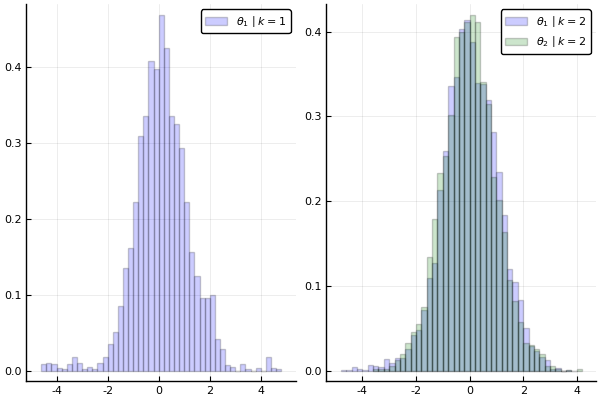
\includegraphics[width=10cm]{images/Reversible.png}
        \caption{Distribution of $\theta$ for each model. The jump
        probability used was 0.1. The distribution for $u$ was a
        standard Cauchy distribution.
        The proportion
        of visits found is 2.47.}
    \end{figure}

    \begin{figure}[H]
        \centering
        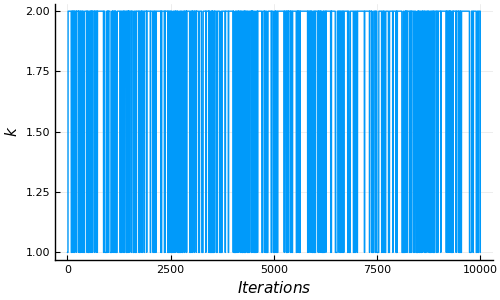
\includegraphics[width=10cm]{images/Jumps.png}
        \caption{Trace plot of the model sampled. It shows that both
        models are well sampled.}
        
    \end{figure}

\newpage
\section*{Simulation question (Reversible jump MCMC)}

The target distribution is $\pi(x) \approx exp(-10(x-1)^2)$.
The tempered distributions are shown in the graph below.

    \begin{figure}[H]
        \centering
        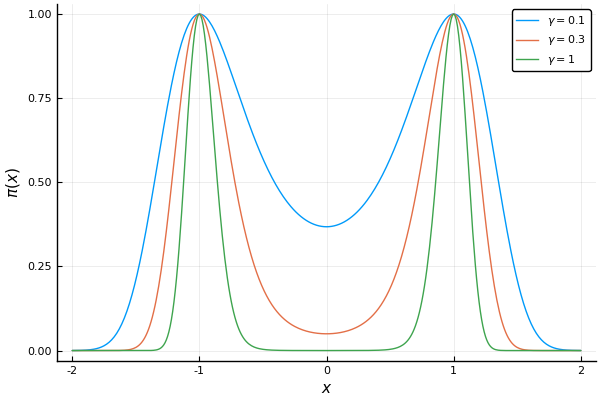
\includegraphics[width=10cm]{images/Tempered.png}
        \caption{Tempered distributions.
        }
    \end{figure}


Looking at the trace plot, for the distributions
with higher $\gamma$ we 
won't get a very good mixture. This problem is not
present when $\gamma$ is lower.

    \begin{figure}[H]
        \centering
        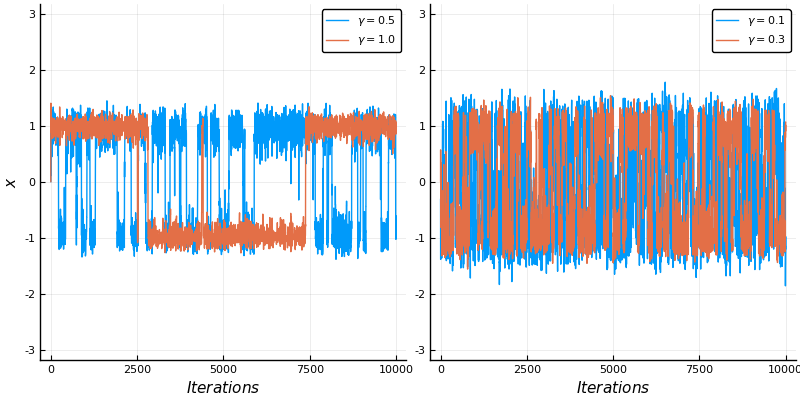
\includegraphics[width=16cm]{images/Trace1.png}
        \caption{Trace plot for different values of tempering.}
    \end{figure}

Implementing the \textit{parallel tempering}, this problem is solved as
can be seen in the figure below.

    \begin{figure}[H]
        \centering
        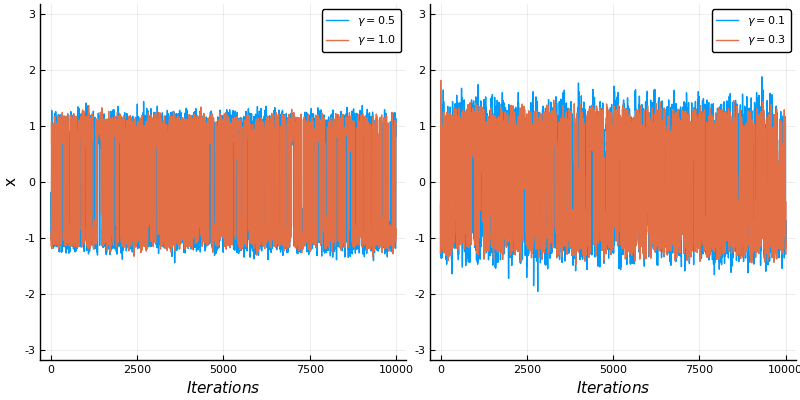
\includegraphics[width=16cm]{images/Trace2.png}
        \caption{Trace plot for the \textit{parallel tempering} model.}
    \end{figure}

\end{document}
